% !TeX program = xelatex
% !TeX encoding = UTF-8
\documentclass[runningheads,orivec]{llncs}
% 必须在加载中文字体前选用 XeLaTeX，避免误用 pdfLaTeX 后查找 unihei 字体。
\RequirePackage{iftex}
\RequireXeTeX
\usepackage[UTF8,scheme=plain,fontset=fandol]{ctex}
\usepackage{amsmath,amssymb,graphicx,booktabs,tabularx,array,longtable}
\usepackage{algorithm,algpseudocode}
\usepackage{tikz}
\usetikzlibrary{arrows.meta,positioning,fit}
\usepackage{url}
% 本地TeX发行版未安装xurl；允许长来源路径在字母和数字间换行。
\makeatletter
\g@addto@macro\UrlBreaks{\do\a\do\b\do\c\do\d\do\e\do\f\do\g\do\h\do\i\do\j\do\k\do\l\do\m\do\n\do\o\do\p\do\q\do\r\do\s\do\t\do\u\do\v\do\w\do\x\do\y\do\z\do\A\do\B\do\C\do\D\do\E\do\F\do\G\do\H\do\I\do\J\do\K\do\L\do\M\do\N\do\O\do\P\do\Q\do\R\do\S\do\T\do\U\do\V\do\W\do\X\do\Y\do\Z\do\0\do\1\do\2\do\3\do\4\do\5\do\6\do\7\do\8\do\9}
\makeatother
\usepackage[hidelinks,unicode,bookmarksdepth=2]{hyperref}
\usepackage{fvextra}
\floatname{algorithm}{算法}
\renewcommand{\figurename}{图}
\renewcommand{\tablename}{表}
\renewcommand{\refname}{参考文献}
\renewcommand{\abstractname}{摘要：}
\renewcommand{\keywordname}{{\bfseries 关键词：}}
\renewcommand{\contentsname}{目录}
\algrenewcommand\algorithmicrequire{\textbf{输入：}}
\algrenewcommand\algorithmicensure{\textbf{输出：}}
\newcommand{\clip}{\operatorname{clip}_{[0,1]}}
\newcommand{\AQ}{\operatorname{AQ}}
\newcommand{\gap}{\operatorname{gap}}
\newcommand{\FE}{\mathrm{FE}}
\newcommand{\JS}{\textsc{GP-J}}
\newcommand{\CT}{\textsc{GP-C}}
\newcommand{\FACO}{\textsc{FACO-N}}
\newcommand{\Ueight}{\textsc{GPU-U8}}
\newcommand{\Usixteen}{\textsc{GPU-U16}}
\newcommand{\Rsixteen}{\textsc{GPU-R16}}
\newcolumntype{L}[1]{>{\raggedright\arraybackslash}p{#1}}
\newcolumntype{Y}{>{\raggedright\arraybackslash}X}
\setlength{\emergencystretch}{1em}
\newcommand{\gentable}[1]{\input{generated/#1.tex}}
\newcommand{\genfigure}[1]{\resizebox{\textwidth}{!}{\input{generated/#1.pgf}}}
\DefineVerbatimEnvironment{TreeCode}{Verbatim}{fontsize=\small,breaklines=true,breakanywhere=true}

\begin{document}
\title{利用Genetic Programming\\学习FACO的搜索控制策略}
\titlerunning{GP学习FACO搜索控制策略}
\author{匿名作者}
\authorrunning{匿名作者}
\institute{}
\maketitle
\begin{abstract}
Focused Ant Colony Optimization（FACO）通过复用参考路径降低构造开销，其搜索表现取决于参考路径、修改起点和扰动强度的选择。本文利用Genetic Programming（GP）学习这些控制决策，将搜索状态与候选动作特征映射为priority scores，并以完整FACO求解的平均终点质量评价规则。研究采用single-tree联合评分和multi-tree条件决策两种表示，在TSP500上分别完成3个GP seed、128个individual、50代训练，再在TSP500和TSP1000上测试冻结策略。TSP500中，两种表示的平均reference gap为0.14759\%和0.15007\%，相对固定MNE=8的GPU对照分别改善0.02183和0.01936个百分点；相对原生FACO适配版及MNE=16对照，差异未达到统计显著。规则分析与决策回放显示，所检查情境中的控制器均选择MNE=16，反馈影响主要体现在区域和重启动作。TSP1000上，固定MNE=16的区域策略取得更低差距；multi-tree也未以较高训练成本换来明确质量收益。实验表明，GP可学习有效的FACO控制规则，而进一步的收益需要超过较强的静态配置，并改善跨规模泛化。
\keywords{Genetic Programming \and FACO \and Hyper-heuristic \and Search control \and TSP}
\end{abstract}
% !TeX root = ../samplepaper.tex
\section{Introduction}
Focused Ant Colony Optimization（FACO）通过复用参考路径的大部分结构，减少旅行商问题（TSP）中重复构造完整路径的开销\cite{skinderowicz2022}。每只蚂蚁只主动引入有限数量的新连接，再由local search改善所得路径。该机制将搜索集中在已有优质解附近，也带来一个控制问题：搜索应从哪里开始、修改多少结构，以及何时转向另一条参考路径？这些决策共同决定了搜索范围和计算工作量。

本文研究利用Genetic Programming（GP）学习上述控制决策。其动机是，固定配置难以区分不同搜索状态：小幅修改可能反复返回参考路径，较大修改则可能增加无效搜索；更换参考路径提供了另一种探索方式，但也会改变可供利用的结构。GP能够以短表达式组合状态与候选动作的特征，形成可在求解过程中反复调用的priority function。离线进化根据完整FACO求解的质量评价这些规则，在线求解则由规则选择动作，蚁群继续负责路径构造与local search。

围绕这一问题，本文定义参考路径切换、起点区域和扰动强度的联合控制接口，并研究single-tree联合评分与multi-tree条件决策两种实现。实验在TSP500上学习策略，通过原生FACO及共享GPU底座的静态策略评价收益，再考察TSP1000迁移、进化规则和计算成本。强度较大的静态策略作为必要对照，用于判断学习所得规则是否超过了简单的参数选择。

\section{Background and Related Work}
\subsection{FACO中的结构复用与控制}
蚁群优化通过信息素积累搜索经验，MAX--MIN Ant System以信息素上下界调节探索与利用\cite{stuetzle2000}。FACO进一步利用参考路径，只主动改变部分连接\cite{skinderowicz2022}。令$q$为参考路径，$P_a$为动作$a$控制的构造过程，$L$为local search，一次候选解生成可表示为
\begin{equation}
 q\xrightarrow{P_a}y\xrightarrow{L}z.
\end{equation}
控制的作用体现在$P_a$生成什么样的候选路径，以及这些候选在$L$之后是否有助于继续改善解。参考路径切换改变$q$，区域选择影响修改起点，MNE（minimum number of new edges）控制主动引入新连接的目标数。MNE不等于最终路径与$q$的边差异数。

后续自适应FACO研究了在线参数调节\cite{skinderowicz2024}。本文的GPU底座采用该后续实现的节点重定位式构造：复制参考路径后，依据候选邻域中的信息素与距离启发式选择节点，再将节点移动到当前节点之后。GP在此基础上学习三项控制的组合。2022原生FACO与该底座的构造和初始化不同，因此实验同时保留原生方法及共享底座的静态对照。

\subsection{GP学习决策规则}
GP hyper-heuristic以启发式规则为搜索对象\cite{burke2013}。一个individual表示priority function；求解过程使用该函数为合法候选评分，并执行排名最高的选择。其fitness来自应用该规则后生成的解。例如，orienteering中的GP对候选访问点评分\cite{mei2018orienteering}，UCARP中的GP学习车辆的任务选择规则\cite{maclachlan2020}。这类方法将规则学习与解的构造连接起来，也便于从表达式分析候选偏好。

当一个求解过程包含多个决策时，multi-tree representation可将不同角色的规则放入同一个individual。Zhang等联合进化routing与sequencing规则，并提出tree-swapping crossover\cite{zhang2018multitree}；Sun等以三棵树分别选择task、cloud和resource，通过共同fitness评价三者的配合\cite{sun2024multicloud}。本文比较完整动作的联合评分与三个控制项的条件选择。二者表达相同类型的控制任务，但具有不同的搜索空间、特征可见性和繁殖方式，实验评价的是这两套完整设计。

% !TeX root = ../samplepaper.tex
\section{Proposed Method}
\subsection{Overview}
方法包含离线进化和在线控制两个过程，如图\ref{fig:overview}所示。离线阶段，GP在多个训练实例上评价控制器：每个individual参与若干次完整FACO求解，所得平均路径质量作为fitness。Selection与genetic operators据此产生下一代。训练结束后，使用validation选择一个individual，作为冻结控制器。

在线阶段，控制器在每次ACO迭代开始时读取当前搜索状态，并选择一个动作。该动作确定本次迭代的参考路径、起点区域和MNE，由整个蚁群共享；各蚂蚁仍独立采样起点和后续节点。构造与local search完成后，求解器更新最优路径、信息素和反馈统计，再进入下一次决策。因此，一棵GP树的输出首先是候选优先级，经过解码得到控制动作，完整求解结束后才能得到fitness。

\begin{figure}[tb]
\centering
\begin{tikzpicture}[x=1mm,y=1mm,>=Stealth,
 every node/.style={font=\small},
 box/.style={draw,align=center,text width=29mm,minimum height=11mm}]
\node[box] (pop) at (0,0) {GP population\\控制规则};
\node[box] (eval) at (40,0) {FACO evaluation\\平均终点fitness};
\node[box] (breed) at (80,0) {Selection\\Genetic operators};
\draw[->] (pop)--(eval); \draw[->] (eval)--(breed);
\draw[->] (breed.north)--++(0,5)-|node[pos=.25,above]{下一代}(pop.north);
\node[box] (state) at (0,-29) {搜索状态\\候选动作特征};
\node[box] (score) at (40,-29) {GP priority scores\\选择$(r,j,k)$};
\node[box] (aco) at (80,-29) {Construction\\Local search};
\draw[->] (state)--(score); \draw[->] (score)--(aco);
\draw[->] (aco.south)--++(0,-7)-|node[pos=.25,below]{更新路径、信息素与反馈}(state.south);
\draw[dashed,->] (eval.south)--node[right,font=\scriptsize]{一次评价中的迭代循环}(score.north);
\end{tikzpicture}
\caption{GP学习FACO控制策略。每个individual在训练实例上执行下方循环，终点质量形成fitness。冻结控制器使用相同的在线循环；参考标签仅由外部评价器读取。}
\label{fig:overview}
\end{figure}

\subsection{Search Decisions and Actions}
求解器维护活动参考路径、全局最优路径、阶段最优路径及容量为4的优质路径archive。Archive保留相对全局最优差距不超过2\%的不同路径。每次决策前，从中选择与活动路径采样边差异最大的合格路径作为备选，并为候选参考路径生成四个起点区域。

动作记为$a=(r,j,k)$。$r\in\{0,1\}$决定保留活动参考路径或切换至备选路径；$j\in\{0,1,2,3\}$决定起点区域；$k\in\{0,1,2,3\}$对应MNE为$2,4,8,16$。区域0和1为参考路径上独立随机抽取的连续片段，区域2沿近邻图广度优先扩展，区域3为不放回随机节点集；每个区域最多16个节点。区域只限制构造的起点，后续修改可以涉及其他节点。

每次迭代最多有32个完整动作。没有合格备选路径时，屏蔽$r=1$的动作。执行参考路径切换时，阶段最优改为备选路径，信息素重新初始化，阶段计数及回归率、local-search工作量的平滑统计清零；全局最优和全局停滞计数保留。当前控制接口没有重启冷却期。

对选定动作，每只蚂蚁复制其参考路径，从所选区域采样起点，完成聚焦构造后执行检查表驱动的2-opt。每只蚂蚁的local search最多评价$10^5$个移动。随后更新archive和反馈，以0.01概率采用阶段最优、否则采用本次迭代最优，作为信息素沉积路径和下一次活动参考路径。完整在线过程见算法\ref{alg:solve}。

\begin{algorithm}[tb]
\caption{FACO求解与GP控制}
\label{alg:solve}
\begin{algorithmic}[1]
\Require 实例$I$，控制器$\pi$，ACO seed $\xi$，蚂蚁数$m$，迭代数$H$
\State 初始化参考路径、信息素、最优路径与archive
\For{$t=1,\ldots,H$}
 \State 读取状态$S_t$，生成合法动作$\mathcal A(S_t)$及特征$\phi(S_t,a)$
 \State $a_t\gets\pi(S_t)$ \Comment{由GP分数解码得到$(r,j,k)$}
 \State 执行参考路径切换，确定起点区域和MNE
 \State 并行构造$m$条候选路径，分别执行local search
 \State 更新最优路径、archive、信息素及搜索反馈
\EndFor
\State \Return 全局最优路径
\end{algorithmic}
\end{algorithm}

\subsection{GP Representation and Decoding}
\paragraph{Joint single-tree（\JS{}）.}
一个individual包含一棵标量树$f$。对每个合法完整动作计算priority score，并选择最高分动作：
\begin{equation}
 \pi_J(S)=\arg\max_{a\in\mathcal A(S)}f\bigl(\phi(S,a)\bigr).
\end{equation}
同一棵树在不同候选特征上重复求值，因而能够比较三项决策的组合。每次决策最多需要32次树求值。

\paragraph{Conditional multi-tree（\CT{}）.}
一个individual包含角色固定的$f_r,f_j,f_k$三棵树，依次完成参考路径、区域和强度选择：
\begin{align}
 r^*&=\arg\max_{r\in\mathcal R(S)} f_r\bigl(\phi_r(S,r)\bigr),\\
 j^*&=\arg\max_{j\in\mathcal J(S,r^*)} f_j\bigl(\phi_j(S,r^*,j)\bigr),\\
 k^*&=\arg\max_{k\in\mathcal K(S,r^*,j^*)} f_k\bigl(\phi(S,r^*,j^*,k)\bigr).
\end{align}
各阶段的候选集合由合法完整动作投影得到；只要一个前缀存在合法补全，便可参与该阶段选择。三次选择读取同一个执行前状态，全部完成后才执行动作。$f_r$可见搜索状态及参考路径特征，$f_j$进一步读取区域特征，$f_k$读取全部输入。最多$2+4+4=10$次树求值即可得到动作。三棵树由同一个fitness共同评价，这与用multi-tree协同学习多个决策规则的GP框架一致\cite{zhang2018multitree,sun2024multicloud}。

\subsection{Terminal Set and Function Set}
表\ref{tab:features}列出12个归一化terminal及其可见性。搜索状态描述当前阶段的进展、停滞和计算反馈；参考路径及区域特征用于区分候选动作。回归率衡量local search后重新得到参考路径的蚂蚁比例，工作量反映搜索所消耗的局部移动评价数。这些反馈为GP提供选择扰动方式的依据。

\begin{table}[tb]
\caption{Terminal set。$\checkmark$表示该角色可以读取；\JS{}读取全部terminal。代码字段及精确归一化公式见补充材料。}
\label{tab:features}
\small
\begin{tabularx}{\textwidth}{@{}lYccc@{}}
\toprule
符号 & 含义 & $f_r$ & $f_j$ & $f_k$\\ \midrule
\multicolumn{5}{l}{搜索状态（search state）}\\
$p$ & Progress：已完成迭代比例$(t-1)/H$ & $\checkmark$ & $\checkmark$ & $\checkmark$\\
$s$ & Stagnation：未改善全局最优的迭代数，按32缩放 & $\checkmark$ & $\checkmark$ & $\checkmark$\\
$\rho$ & Return rate：返回参考路径的蚂蚁比例，平滑后使用 & $\checkmark$ & $\checkmark$ & $\checkmark$\\
$w$ & LS work：每蚂蚁平均局部移动评价数，按$10^5$缩放并平滑 & $\checkmark$ & $\checkmark$ & $\checkmark$\\
\midrule
\multicolumn{5}{l}{参考路径与动作（reference and action）}\\
$r$ & 候选动作的参考路径切换标记 & $\checkmark$ & $\checkmark$ & $\checkmark$\\
$\delta_q$ & 候选参考路径相对全局最优的差距，按0.02缩放 & $\checkmark$ & $\checkmark$ & $\checkmark$\\
$d_q$ & 候选与活动参考路径的采样边差异 & $\checkmark$ & $\checkmark$ & $\checkmark$\\
$u$ & MNE level：$(k+1)/4$，即0.25、0.5、0.75、1 & & & $\checkmark$\\
\midrule
\multicolumn{5}{l}{候选区域（candidate region）}\\
$e_R$ & Region excess：相邻边相对近邻距离的长度超额 & & $\checkmark$ & $\checkmark$\\
$a_R$ & Archive disagreement：区域相邻边在archive中的缺失比例 & & $\checkmark$ & $\checkmark$\\
$\tau_R$ & Pheromone strength：区域相邻边的归一化信息素 & & $\checkmark$ & $\checkmark$\\
$d_R$ & Region dispersion：相邻端点落在区域外的比例 & & $\checkmark$ & $\checkmark$\\
\bottomrule
\end{tabularx}
\end{table}

两种表示使用相同的function set：$+$、$-$、$\times$、$\min$、$\max$、绝对值及analytic quotient，后者定义为$\AQ(a,b)=a/\sqrt{1+b^2}$。常量terminal包括$-1,0,1$及从$[-2,2]$均匀采样的ephemeral random constants（ERC）。比例特征裁剪至$[0,1]$，两个平滑反馈采用权重$1/16$的指数移动平均。

实际树求值使用FP32，每个运算结果裁剪至$[-8,8]$。分数差不超过$10^{-6}$时，选择编号最小的合法候选；完整动作按$16r+4j+k$编号。这些规则确定近并列情况下的行为，解释表达式时同时保留其数学形式与实际解码结果。

\subsection{Fitness Evaluation and Evolution}
GP优化控制器在完整求解结束时的路径质量。设$\mathcal B_g$为第$g$代共享的实例--ACO seed面板，$T(I,\xi;\pi)$为算法\ref{alg:solve}返回的路径，$C_{\rm ref}(I)$为外部评价器读取的参考路径长度，则最小化
\begin{equation}
 F_g(\pi)=\frac{1}{|\mathcal B_g|}\sum_{(I,\xi)\in\mathcal B_g}
 100\left(\frac{C(T(I,\xi;\pi))}{C_{\rm ref}(I)}-1\right).
 \label{eq:fitness}
\end{equation}
该值以百分数表示，称为reference gap。参考路径未逐例独立认证最优性。参考标签不进入控制器输入或FACO求解。每代更换训练面板，同代所有individual及两种表示的运行共享面板，elites也重新评价。训练实例轮换在GP规则学习中已有应用\cite{mei2018orienteering,maclachlan2020}；本实验通过固定validation面板观察其学习表现。

初始化按目标高度2、3、4及full/grow方式分层采样；grow保留一条达到目标高度的分支。每棵树高度至多5，每个individual总节点数至多63，三树共享总节点限制。父本通过tournament selection选取。Crossover以0.9概率选择非terminal位置，并允许选择根；single-tree将第二父本的子树接入第一父本。Multi-tree先随机选择一个角色进行同角色subtree crossover，其余角色整树取自第二父本。该操作同时重组角色内部结构和角色间组合，与tree-swapping crossover属于相关设计\cite{zhang2018multitree}。

Mutation替换一个随机角色中的子树；对单叶树采用生长变异。每代保留elites，并以crossover、mutation或reproduction产生其余individual。为维持搜索多样性，接受的程序须互异，在64个固定训练情境上产生相同动作向量的individual最多两个。超出结构限制或重复的候选重新生成，必要时采用随机移民。具体概率、重试范围与精确语义列于实验设置及补充材料。

\begin{algorithm}[tb]
\caption{GP控制器的离线学习}
\label{alg:gp}
\begin{algorithmic}[1]
\Require 表示类型，GP seed，训练面板$\{\mathcal B_g\}_{g=1}^G$，validation面板
\State 初始化$P$个满足结构和行为约束的individual
\For{$g=1,\ldots,G$}
 \State 在$\mathcal B_g$上执行算法\ref{alg:solve}，按式\eqref{eq:fitness}评价整个种群
 \State 保存本代冠军，并按固定间隔在开发面板上监控
 \If{$g<G$}
  \State 保留elites，通过selection与genetic operators补齐下一代
 \EndIf
\EndFor
\State 对历代冠军与末代种群执行两级validation，选择并冻结一个控制器
\State \Return 冻结控制器
\end{algorithmic}
\end{algorithm}

\subsection{Parallel Fitness Evaluation}
Fitness evaluation将individual、实例／ACO seed和ant三个维度展开至GPU。不同蚁群分别维护路径、信息素、archive和随机流；实例几何量复用，GP树编译为紧凑指令执行。不同GP seed和独立评价任务分配至空闲RTX A5000。路径几何、代价和local-search增益使用FP64。

一次蚂蚁路径构造及其local search记为一次evaluation（FE），一次求解的预算为$mH$。此预算限制候选路径数；不同控制策略仍可能消耗不同数量的构造步和局部移动评价。因此，实验分别报告FE、搜索工作量及GPU时间。

\section{实验设计}
\subsection{数据、参数依据与分阶段预算}
主实验只在500节点欧氏TSP上训练，1000节点实例仅用于冻结后的规模迁移测试。实例、参考路径和面板归属由现有数据清单固定，清单将该合成实例族记为uniform。现存元数据没有完整记录生成器及父实例关系，本文不额外假定未记录的生成过程。参考路径是数据集提供的比较基准，未逐例独立认证最优性。对路径$T$，评价指标为
\begin{equation}
 \gap(T)=100\left(\frac{C(T)}{C_{\mathrm{ref}}}-1\right)\%,
\end{equation}
其中$C$按连续欧氏距离计算。文中称其为\emph{参考差距}，而非已认证最优差距。标签仅由外部评价器读取，以高精度求和计算长度；在线求解器不读取标签或标签路径。

蚂蚁数采用2022 FACO实验的规模规则$m=64\lceil\sqrt n/16\rceil$\cite{skinderowicz2022}，TSP500和TSP1000均为128。主要／备用候选数16／64、局部搜索候选数20、$\beta=1$、信息素保留系数0.5、$p_{\mathrm{best}}=0.1$、阶段最优使用概率0.01在GPU方法间固定。MNE8作为FACO式默认强度对照，MNE16用于排除最大强度本身带来的收益。GP种群、节点上限和算子概率是控制搜索规模的实验设计选择，并未经过全面超参数优化。

训练迭代数允许少于测试，但不按时间截断。先前开发标定比较24个固定或规则控制器，使用32个开发实例与5个ACO种子，在候选$H\in\{100,250,500,1000,2500,5000\}$上要求保留至少95\%的相对初始化改善，且与$H=5000$的控制器排名Spearman相关至少0.9。TSP500中，$H=1000$是首个同时达标的候选，改善保留率为98.73\%，排名相关为0.9383。此依据来自开发控制器，并不保证进化GP在短、长预算下排名一致。

表\ref{tab:protocol}给出正式轮次预算。三种GP种子为1103、2207、3313，每种表示各运行一次，共6次。所有运行在同一代共享实例与ACO随机种子面板，训练面板随代变化，50个面板合计覆盖794个不同训练实例。监控、选模和测试均不含这些训练实例，快速验证与完整验证的实例也不重叠。每个个体每代$16\times1\times128\times1000=2{,}048{,}000$ FE，每次50代训练为$13{,}107{,}200{,}000$ FE；六次合计$78{,}643{,}200{,}000$ FE，不含监控、选模和测试。

\begin{table}[tb]
\caption{正式实验流程。每次求解均使用128只蚂蚁；快速与完整验证使用不同面板。}
\label{tab:protocol}
\small
\begin{tabularx}{\textwidth}{@{}lrrY@{}}
\toprule
阶段 & 实例$\times$ACO种子 & $H$ & 评价对象与用途\\ \midrule
训练 & $16\times1$ & 1000 & 每代128个体，50代，面板随代变化\\
开发监控 & $16\times1$ & 1000 & 第5、10、$\ldots$、50代冠军；固定面板\\
快速验证 & $32\times1$ & 1000 & 历代冠军与末代种群，去重后最多177个\\
完整验证 & $64\times3$ & 5000 & 每次运行快速验证前4名，选出1个\\
TSP500测试 & $128\times10$ & 5000 & 六个冻结控制器及四种对照\\
TSP1000测试 & $128\times10$ & 5000 & 原样迁移，不重新进化或选模\\
\bottomrule
\end{tabularx}
\end{table}

监控和快速验证的ACO种子为17；完整验证为17、29、41；测试为17、29、41、53、67、79、97、109、127、149。划分以实例清单为准，重复使用种子编号不意味着重复使用测试实例。六个控制器全部冻结后才执行正式测试。本次整理没有新增ACO评价，也没有根据测试结果修改方法。

\subsection{对照与统计方法}
四种对照分别为：\FACO{}，保留24条初始化路径的原生2022 FACO；\Ueight{}，GPU底座、MNE8、全体节点均匀起点且不重启；\Usixteen{}，仅将前者强度改为16；\Rsixteen{}，GPU底座、MNE16、每迭代随机生成的区域0起点且不重启。区域0对照可以检验局部起点限制是否已足以解释收益。GPU静态对照与GP使用相同构造、局部搜索及数值后端。

\FACO{}在合成数据上使用连续FP64距离，并将依赖距离取整的KD-tree邻域实现替换为近邻列表；对恒等2-opt移动赋零增益，并排除边集合不变的3-opt移动，以避免浮点误差触发虚假改善循环。它应理解为原生FACO的连续距离适配版。另有保留原始整数距离的TSPLIB\cite{reinelt1991}复现实验，详见补充材料；二者不合并为同一结果。

质量均值先对ACO种子求平均，再对实例和GP种子求平均。主检验以128个测试实例为配对单位，每个实例先平均10个ACO种子与3个GP种子，采用双侧Wilcoxon符号秩检验\cite{wilcoxon1945}。TSP500预定的9项比较为两种GP各对四种对照及GP之间比较，统一进行Holm校正\cite{holm1979}。95\%区间采用10\,000次分层配对bootstrap，重采样GP种子、实例及实例内ACO种子，统计种子为91001。定义改善$\Delta=\gap_{\text{对照}}-\gap_{\mathrm{GP}}$，以百分点报告，正值表示GP更好。TSP1000区间作为迁移效果的描述性证据，不额外扩展主检验族。3个GP种子仍限制了对进化随机性的估计精度。

% !TeX root = ../samplepaper.tex
\section{Results and Analysis}
\subsection{RQ1: Performance on TSP500}
两种GP控制器均改善了默认强度对照的求解质量。表\ref{tab:quality}中，\JS{}与\CT{}的平均reference gap分别为0.14759\%和0.15007\%，\Ueight{}为0.16942\%。对应改善为0.02183和0.01936个百分点，Holm校正后的$p$值分别为0.00015和0.00006，95\%区间均高于零（图\ref{fig:effects}）。这说明在相同底座与FE预算下，GP能够学到优于该静态配置的控制规则。

\begin{table}[tb]
\caption{冻结测试的平均reference gap（\%，越低越好）。每个规模128个实例、10个ACO seed；GP结果再平均3个GP seed。}
\label{tab:quality}
\centering\gentable{quality}
\end{table}

较强静态策略缩小了GP的优势。\Rsixteen{}与\Usixteen{}的gap为0.15163\%和0.15406\%，接近两种GP；这些配对差异的区间均跨越零，校正后未达到统计显著。相对\FACO{}的均值也有所降低，但没有得到显著差异。因此，现有结果支持GP超过MNE=8配置，尚不足以说明其稳定优于原生FACO适配版或MNE=16配置。下一节结合规则分析考察GP是否主要偏好较大扰动。

\begin{figure}[tb]
\centering\genfigure{effects}
\caption{相对各对照的gap改善及95\%分层配对bootstrap区间，单位为百分点。点在零线右侧表示GP更好；标签为“方法／对照”。星号仅标记TSP500九项Holm校正后$p<0.05$的比较；TSP1000为描述性区间。}
\label{fig:effects}
\end{figure}

本文用绝对百分点描述这些收益。例如，\JS{}相对\Ueight{}的逐求解平均路径长度改善约为0.02165\%；它与reference gap均值相对下降约12.9\%是不同量。后者表示剩余差距的缩小比例。

\subsection{RQ2: Learning Behaviour and Evolved Rules}
\paragraph{学习过程与选模.}
固定validation面板显示，两种表示随训练有小幅改善，但波动仍较大。图\ref{fig:curves}的下排使用训练结束后对每代冠军的quick-validation重评；按10代窗口平均，\JS{}从前10代的0.24250\%降至后10代的0.23166\%，\CT{}从0.24669\%降至0.22815\%。上排则以同代\Rsixteen{}为参照，消除部分训练面板难度变化。两种表示在TSP500测试中的差异为0.00247个百分点，区间跨零，未显示明确的表示优势。

\begin{figure}[tb]
\centering\genfigure{curves}
\caption{Training与quick validation。列分别为\JS{}和\CT{}；细线为三个GP seed，粗线为均值，均未平滑。上：训练冠军相对同代\Rsixteen{}的改善，正值更好；下：固定quick-validation面板重评的冠军gap，越低越好。下排在训练结束后计算，H1000，与最终选模的H5000 full validation不同。}
\label{fig:curves}
\end{figure}

Full validation所选的六个individual均不是末代训练冠军，只有两个是quick validation第一名。例如，\JS{}的seed 1103中，quick validation第四名在full validation达到0.12667\%，优于第一名的0.14551\%。这表明在当前设置下保留多个候选参与较长预算选模是有用的。两个validation阶段同时改变实例、ACO seed数和迭代预算，排名反转反映它们的综合影响。

末代种群仍保留结构和行为差异：每次运行有128个不同程序，在64个固定训练情境中产生100--115种动作向量；最大树高的中位数为4--5。不同fitness值有104--121个，说明终点评价可以区分多数individual。该训练信号仍是完整求解后的单个标量，多次在线决策及multi-tree的不同角色共同承担credit assignment。

\paragraph{从表达式理解控制偏好.}
六个选中individual包含5--35个节点。图\ref{fig:decoding}以两个seed 3313控制器展示规则如何得到动作；示例用于解释其结构与语义，全部六个individual见补充材料。\JS{}中最短的规则为
\begin{equation}
 f=\AQ\bigl(u,\AQ(\rho,d_R)\bigr).
 \label{eq:joint-rule}
\end{equation}
对固定区域，该式随MNE level $u$增大而增大，因此偏好MNE=16。当$\rho>0$时，较大的$d_R$使内层AQ减小、外层得分增大，规则倾向选择相邻端点更多落在区域外的起点集合。$\rho$接近零时，不同区域的分数差也趋小，实际选择可能由并列规则决定。

\begin{figure}[tb]
\centering
\begin{minipage}[c]{0.38\textwidth}\centering\small
\textbf{GP-J/3313}\par\medskip
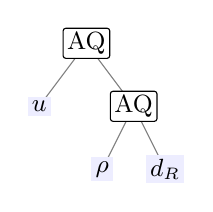
\begin{tikzpicture}[x=8mm,y=8mm,every node/.style={font=\small,inner sep=1.5pt}]
\draw[gray] (1.5,-1) -- (1,-2);
\draw[gray] (1.5,-1) -- (2,-2);
\draw[gray] (0.75,0) -- (0,-1);
\draw[gray] (0.75,0) -- (1.5,-1);
\node[fill=blue!7] at (0,-1) {$u$};
\node[fill=blue!7] at (1,-2) {$\rho$};
\node[fill=blue!7] at (2,-2) {$d_R$};
\node[draw,rounded corners=1pt,fill=white] at (1.5,-1) {$\AQ$};
\node[draw,rounded corners=1pt,fill=white] at (0.75,0) {$\AQ$};
\end{tikzpicture}
\par\medskip
\end{minipage}\hfill
\begin{minipage}[c]{0.59\textwidth}\centering\small
$\rho=0.00746447$，$u=1$\par
保留参考路径时：\par\smallskip
\begin{tabular}{cr}\toprule 区域$j$ & MNE16得分\\\midrule
0 & 0.999972165\\
1 & 0.999972165\\
2 & 0.999972999\\
3 & 0.999985993\\
\bottomrule\end{tabular}\par\smallskip
输出：$(r,j,\mathrm{MNE})=(0,3,16)$
\end{minipage}

\caption{选中规则与真实解码示例。左：\JS{}/3313的完整5节点树；右：\CT{}/3313的三棵树表达式及条件选择流程。下方给出两者各自在TSP500首个解释实例、ACO seed 17、第100迭代的分数；两条运行轨迹的状态不同。候选按编号排序，分数直接取自保存的CUDA回放。}
\label{fig:decoding}
\end{figure}

\CT{}/3313将三项决策分开，其区域规则为$p+\max(p,a_R\tau_R)$。同一决策状态中的$p$对各区域相同，因此区域偏好来自archive disagreement与pheromone strength的乘积：当乘积超过$p$时，该区域获得更高分。其强度规则为$u+(p+\rho)$，后两项是候选间的公共偏置，MNE排序由$u$决定。另两个\CT{}控制器的强度树在当前输入域内也偏好最大$u$。这些例子说明，表达式包含反馈terminal，并不意味着每项决策都随反馈改变。

\paragraph{观测动作与反馈响应.}
表达式中的强度偏好与已有回放一致。六个控制器在64个训练情境上共384次决策，以及两个规模的开发实例回放共144次决策，全部选择MNE=16。真实回放覆盖每规模2个实例和6个迭代位置；这些记录提供了策略行为的样本。

将停滞、回归率或工作量分别设为0或1后，MNE仍未变化，但部分区域与重启动作发生变化。图\ref{fig:decoding}中，\CT{}/3313的参考路径得分包含$w$与$s$，而强度树的反馈项是公共偏置，体现了反馈在不同角色中的不同作用。该诊断只改变固定状态下的输入，并未重新运行FACO，所以衡量的是动作敏感性。

完整测试的累计重启数进一步显示策略间差异。TSP500中，\JS{}三个控制器每5000迭代平均重启0、402.8、492.8次，\CT{}分别为433.8、231.4、726.4次。较高频率与当前接口缺少冷却期相符。结合静态MNE=16对照，后续需要通过完整求解实验分离区域选择与参考路径切换的收益；现有评分诊断尚不能回答这两部分是否改善了终点质量。

\subsection{RQ3: Transfer and Computational Cost}
TSP500训练所得策略在TSP1000上仍优于\Ueight{}的均值，但没有超过较强区域策略。\Rsixteen{}的reference gap为0.22825\%，低于\JS{}的0.25236\%和\CT{}的0.24563\%。两种GP相对它的改善分别为$-0.02411$和$-0.01738$个百分点，描述性95\%区间均位于零以下（图\ref{fig:effects}）。该结果表明，在当前测试族中，归一化特征和相同动作接口尚未使学习策略在更大规模上保持相对强静态对照的优势。

\begin{table}[tb]
\caption{计算成本。训练及监控／选模为每次GP运行的平均GPU任务分钟；测试列为TSP500每1280次求解的批处理摊销时间总和及每FE的平均LS移动评价数，GP再平均3个seed。静态策略不需要GP训练。}
\label{tab:maincost}
\centering\small\gentable{maincost}
\end{table}

\CT{}的训练成本高于\JS{}，而两者测试质量接近。表\ref{tab:maincost}中，平均训练GPU时间分别为393.21和283.72分钟，相差38.6\%；监控加选模约占训练的10.7\%和11.3\%。因此，当前conditional representation减少了每次决策的树求值次数，却没有降低完整训练成本。动作还会影响构造、local search和重启工作量，树求值次数只反映成本的一部分。

在两个测试规模上，GP的摊销GPU时间为\Ueight{}的约1.29--1.73倍，LS移动评价数为其约1.52--1.80倍。相同FE预算下，较高强度的搜索仍会消耗更多计算。已有同卡布局优化在四组种群样本上减少10.7\%--14.4\%的评价时间，细节列于补充材料。这里的GPU任务时间用于描述批处理成本，训练墙钟时间另列；不同服务器及CPU原生对照不用于计算直接加速倍数。

% !TeX root = ../samplepaper.tex
\section{Conclusion}
本文从local search的候选起点出发设计FACO外层控制，将参考路径切换、扰动起始区域和强度联合表述为GP可学习的决策。在固定构造与local-search组件下，TSP500上的两种表示均学到优于MNE=8配置的规则，但MNE=16静态对照取得接近质量，TSP1000上的区域静态策略进一步超过两种GP。规则分析与采样决策显示对MNE=16的偏好，反馈主要影响区域和重启动作。质量改善伴随着更多LS工作；multi-tree也未以更高训练成本换来明确质量收益。

这些结果支持围绕local search考察外层控制，同时将尚待验证的问题集中到状态相关决策的增量价值。后续应在另行划定的预实验实例集固定MNE=16，对反馈、区域选择及参考路径切换进行完整求解消融，联合测量终点质量与LS工作量，并检查停滞特征、重启频率及训练与部署预算的差异。现有scalar fitness由多个决策共同承担credit assignment，动作敏感性还不足以分离各项控制的质量贡献。结论来自三个GP seed、TSP500训练与TSP1000迁移；FACO面向大规模问题的设计背景不等同于本方法已完成大规模泛化验证。

\bibliographystyle{splncs04}
\bibliography{references}
\end{document}
